\documentclass[11pt, xcolor=dvipsnames]{beamer}
\usepackage[utf8]{inputenc}
\usepackage[T1]{fontenc}
\usepackage{lmodern}
%\usetheme{Madrid}
\usetheme{CambridgeUS}
%\useoutertheme{miniframes}

\usepackage{xcolor} % Required for specifying colors by name
\usepackage{multicol} 
\usepackage{graphicx}
% Define custom colors
% link for more colors: http://latexcolor.com
\definecolor{UTEPorange}{rgb}{255, 130, 0} % primary
\definecolor{UTEPblue}{rgb}{4, 30, 66}
\definecolor{UTEPsilver}{rgb}{177, 179, 179}
\definecolor{raspberry}{rgb}{0.89, 0.04, 0.36}

%\setbeamercolor{palette primary}{bg=gray, fg=white}
%\setbeamercolor{palette secondary}{bg=UBCblue,fg=white}
%\setbeamercolor{palette tertiary}{bg=UBCblue,fg=white}
%\setbeamercolor{palette quaternary}{bg=UBCblue,fg=white}
%\setbeamercolor{structure}{fg=UBCblue} % itemize, enumerate, etc
%\setbeamercolor{section in toc}{fg=UBCblue} % TOC sections


\usecolortheme[named=raspberry]{structure}

\begin{document}
	\title[Chicago Bike-sharing Network Analysis ]{Divvy (Chicago) Bike-sharing Network Analysis}
	\subtitle{}
	\logo{\href{https://www.utep.edu}{
\includegraphics[height=0.75cm]{utep-logo.png}}}
	\author[William Agyapong]{By:\\ \textit{William Agyapong }}
	\institute{\href{https://www.utep.edu}{University of Texas at El Paso}\\ Department of Mathematical Sciences}
	\date{\today}
%	\subject{}
	\setbeamercovered{transparent}
	\setbeamertemplate{navigation symbols}{}
	
	\setbeamertemplate{footline}{
		
		\begin{beamercolorbox}[ht=0.30cm,leftskip=0.3cm,rightskip=.3cm]{author in head/foot}
			\usebeamercolor{red}
			\usebeamerfont{section in head/foot}
			%		\linethickness{0.25pt}
			%		\hrule
			\insertshortauthor~-~\insertshorttitle 
			\hfill 
			\insertframenumber/\inserttotalframenumber
			
		\end{beamercolorbox}
	}

	\begin{frame}[plain]
				\begin{columns}[T]
					\begin{column}{0.5\textwidth}
							\vspace{0.2\linewidth}
							\maketitle
					\end{column}
					\begin{column}{0.5\textwidth}
						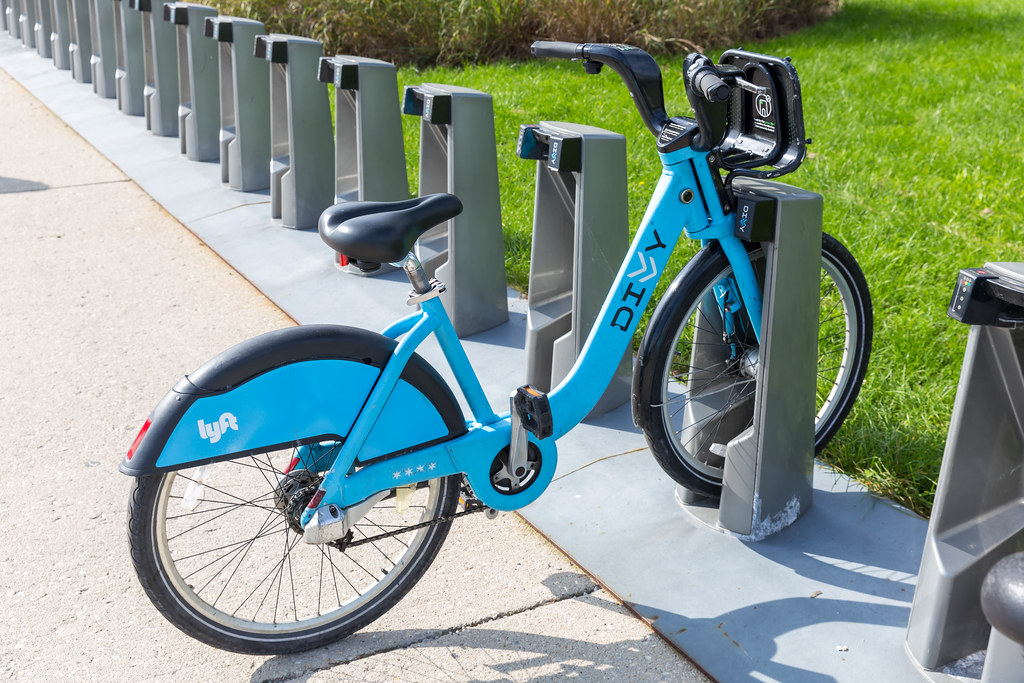
\includegraphics[width=7cm, height=9cm]{images/divvy-3}
					\end{column}
				\end{columns}
	\end{frame}

%    \frame{
%    	\titlepage 
%    }
%	 \frame{\tableofcontents}
	 \begin{frame}{Outline}
	 		\begin{columns}[T]
	 		\begin{column}{0.5\textwidth}
	 			\vspace{0.3\linewidth}
	 			\tableofcontents
	 		\end{column}
	 		\begin{column}{0.5\textwidth}
	 			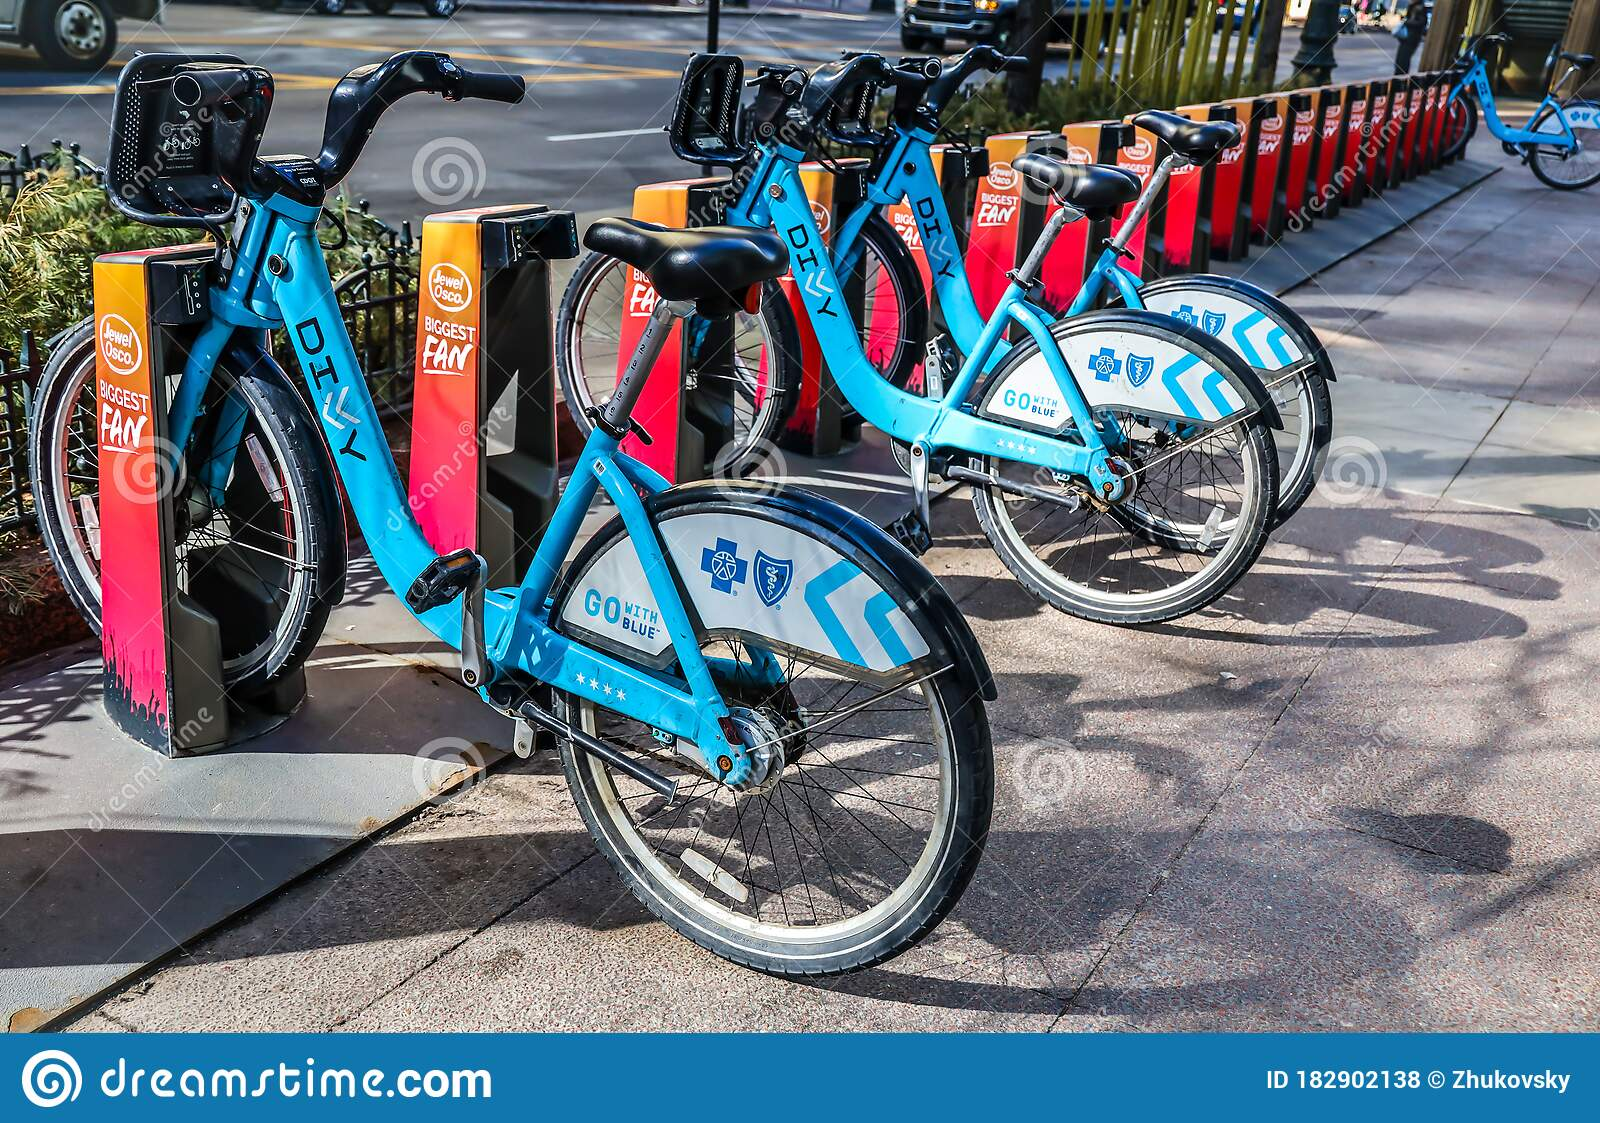
\includegraphics[width=7cm, height=9cm]{images/chicago-illinois}
	 		\end{column}
	 	\end{columns}
	 \end{frame}
	\section{Introduction}
		\subsection{Background and Motivation}
	\begin{frame}{A little about DIVVY, the Chicago Bike-share System}
		\centering
		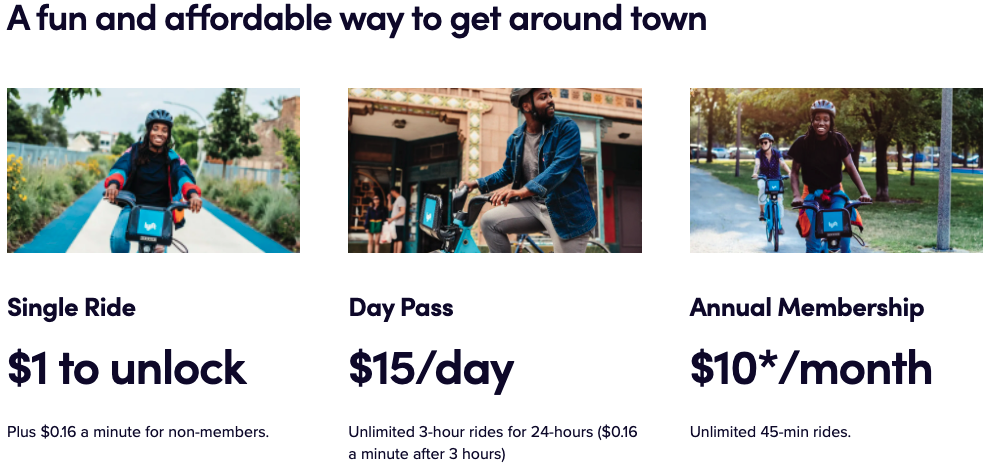
\includegraphics[width=11cm]{images/divvy-about}\\ % information as at May 7, 2022 8:30 MT
		 Divvy is a playful reference to sharing ("divvy it up"). Divvy’s light-blue color palette and four stars evoke the Chicago flag. The double Vs in the Divvy logo refer to the shared-lane markers painted on bike lanes throughout the city, showing how the city prioritizes bike safety.
	\end{frame}

    \begin{frame}{How it works}
    	\centering
    	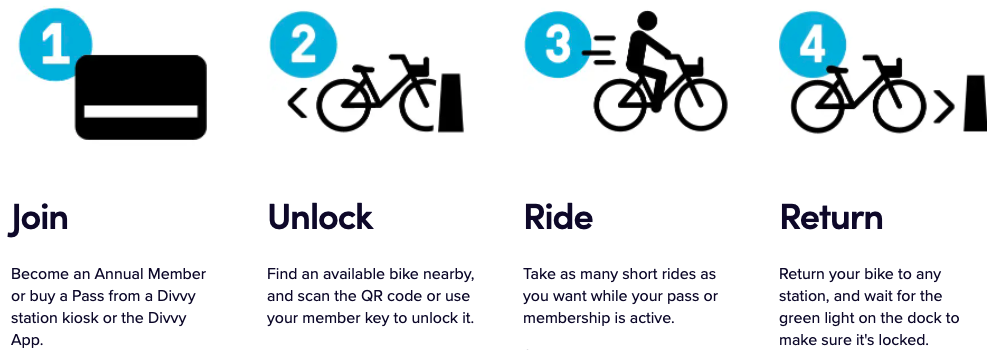
\includegraphics[width=12cm]{images/how-it-works-2}
    \end{frame}
	\begin{frame}{Background and Motivation}
		\begin{itemize}
			\item Safety, health, economic and environmental benefits
			\item Much focus placed on the use of network analysis methodologies.
			\item Yao etal. (2019) employed complex network methods to analyze the relationship between stations within theNanjing bike-sharing system in China.
			\item Rixey (2013) also expanded on prior studies involving the use of station-level ridership data by including the network effects of the size and spatial distribution of the bike sharing station network
		\end{itemize}
	\end{frame}
		\subsection{Main objectives}
		\begin{frame}
			\frametitle{Objectives of the project}
			The study seeks to address the following research questions:
			\begin{itemize}
				\item Do different user types (members or casual users) and bike rideable types (classic, docked, and electric bikes) influence ridership in general and in terms of network structure?
				
				\item What are the central stations within the bike-share system station network?
				
				-\item Is there some underlying community structure that can be utilized by the operators of the Chicago public bike-share system to help meet operational needs as well as the needs of bike riders?
			\end{itemize}
		\end{frame}
	\subsection{Data Exploration}
	 \begin{frame}{Data Exploration}
	 	\begin{itemize}
	 		\item Downloaded directly from the Divvy system data repository
	 		\item 5,757,551 observations measuring the total number of trips over a 12-month period
	 		\item $10\%$ stratified random sample  was taken
	 		\item Final study size of 455275 after treating data anomalies
	 	\end{itemize}
 	\centering
 	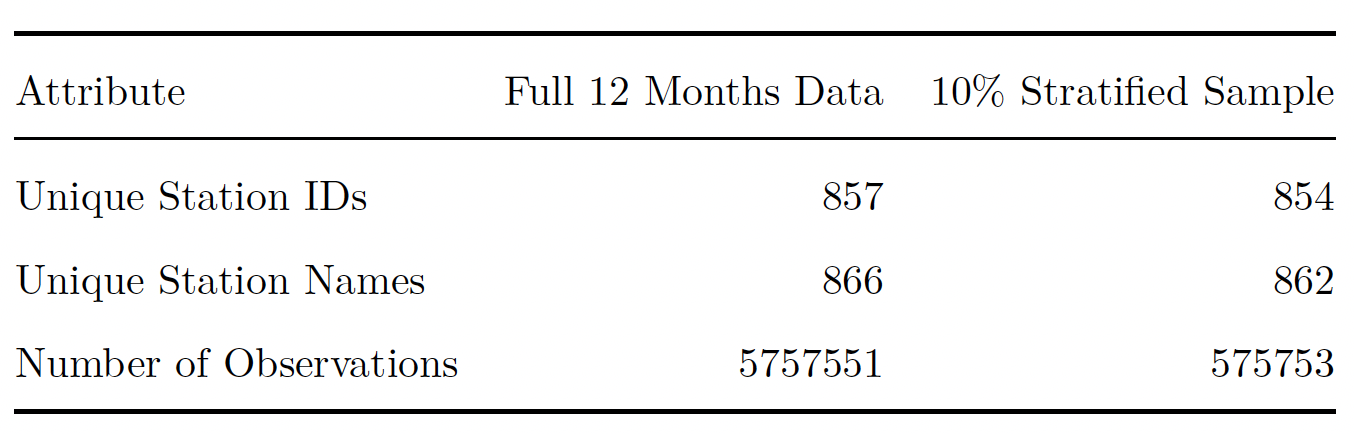
\includegraphics[width=9cm]{images/fulldata-vs-stratified}
 	
	 \end{frame}
 
    \begin{frame}{Data Exploration: Variables}
   	  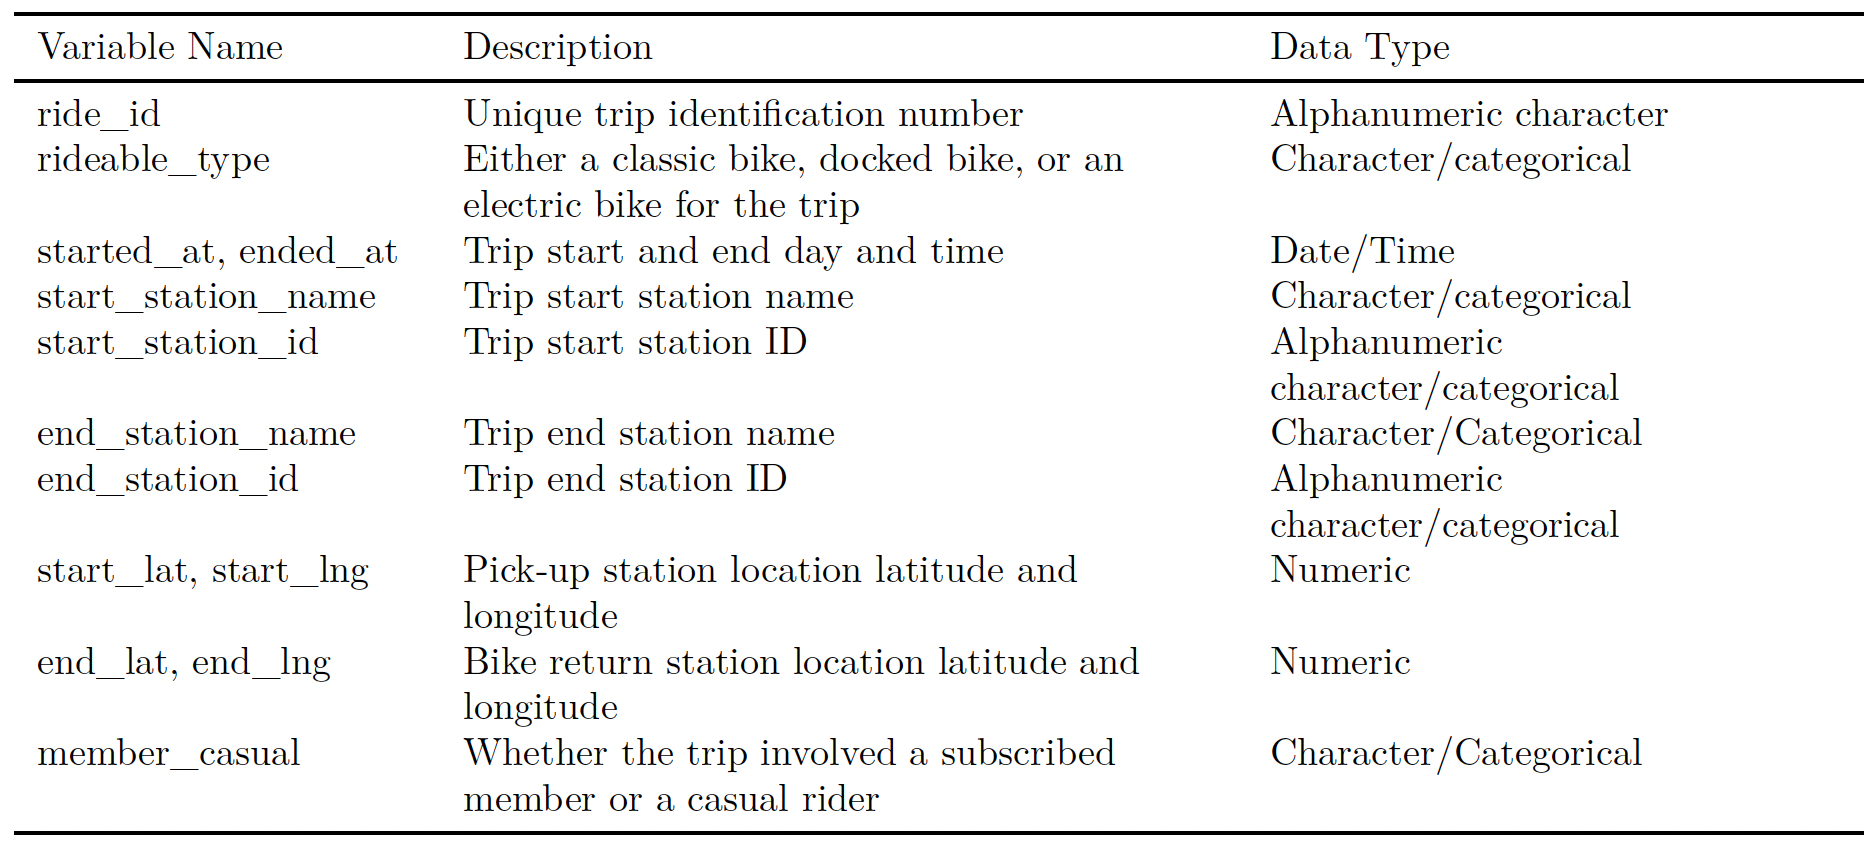
\includegraphics[width=12cm]{images/variables}
    \end{frame}

   \begin{frame}{Trip Time length Anomalies}
  			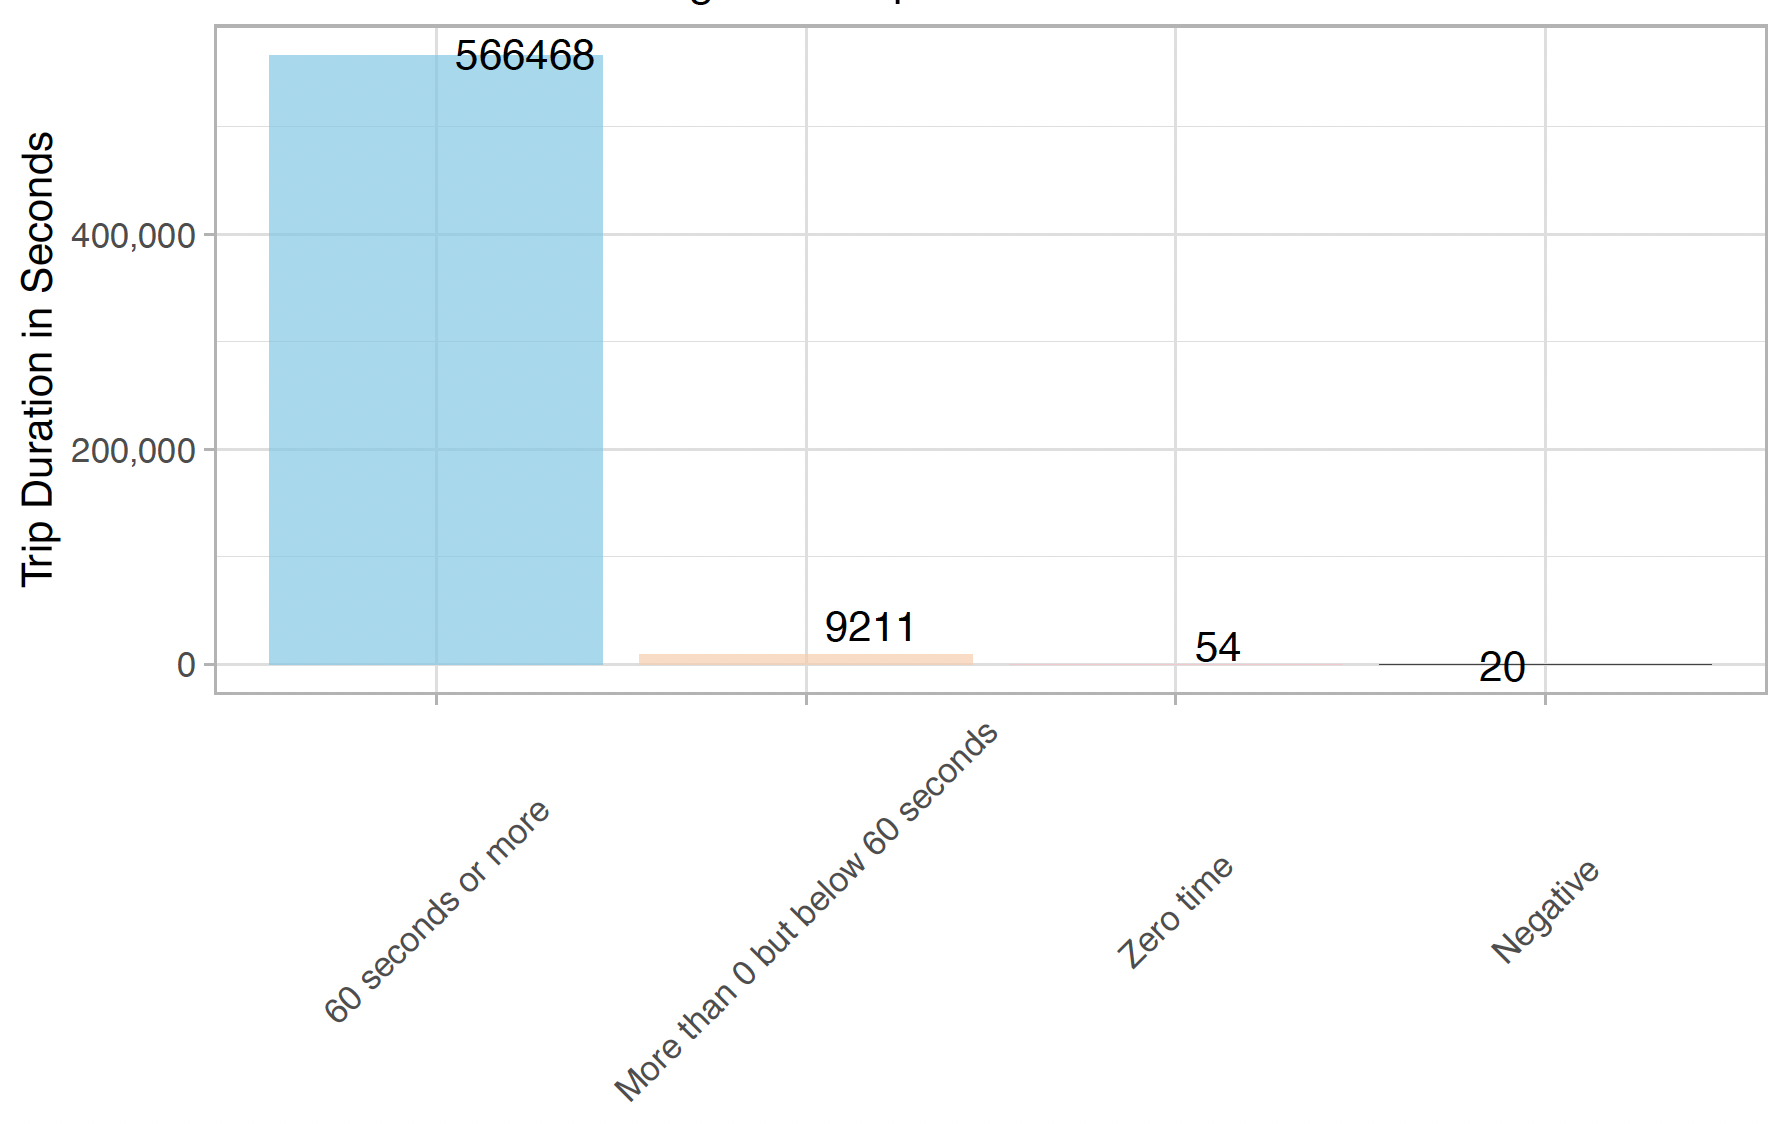
\includegraphics[width=12cm]{images/time-anomaly}
   \end{frame}
 
  
	\section{Methodology}
	\subsection{Sampling framework and Graph theory concepts}
	
	\begin{frame}{Methods Used}
		\begin{itemize}
			\item Stratified Random Sampling
				\item Centrality measures: Degree and Betweenness
			
			\item Interconnectivity measures: 
			\begin{itemize}
				\item Average path length
				\item Diameter
				\item Density
			\end{itemize}
		  \item Community Detection Algorithms:
		   	\begin{itemize}
		   		\item Louvain Algorithm
		   		\item Walktrap Algorithm
		   	\end{itemize}
%	   	  \item Modularity Score
		\end{itemize}
	\end{frame}
	\section{Results}

	\begin{frame}{Distributions of Rides by day of week and type of bike users}
		\centering
		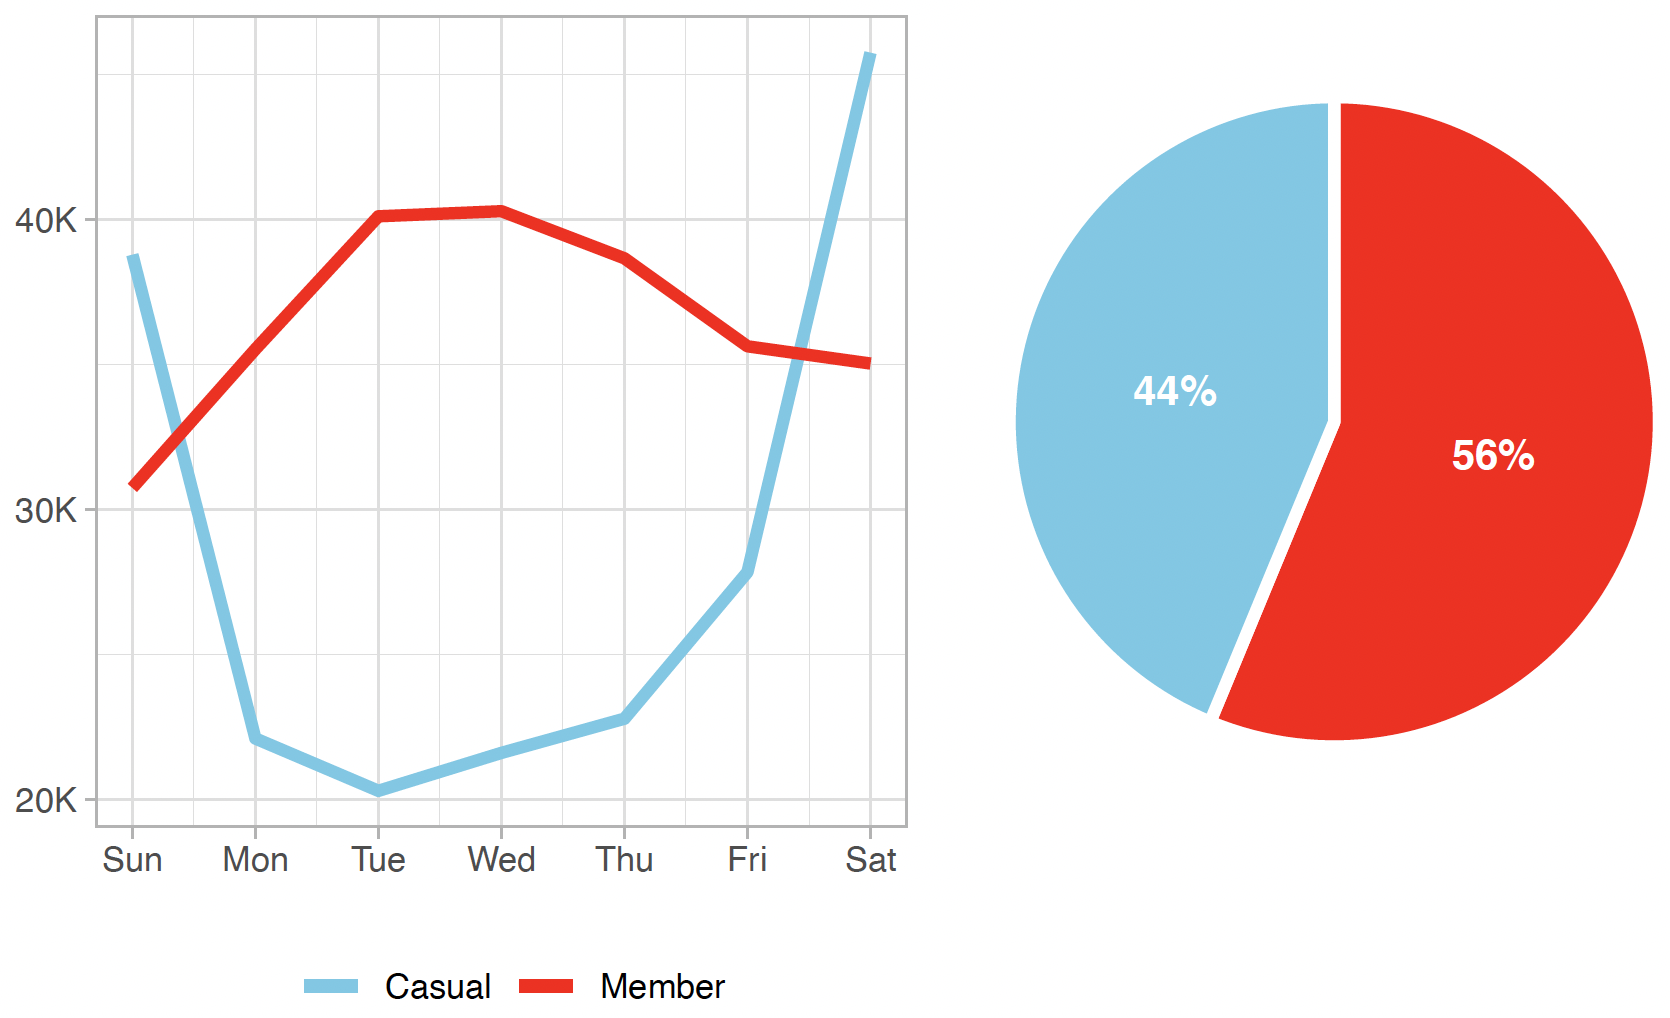
\includegraphics[width=11cm, height=7cm]{images/member-casual-dayofweek}

	\end{frame}

	\begin{frame}{Distributions of Rides by day of week and rideable types}
	\centering
	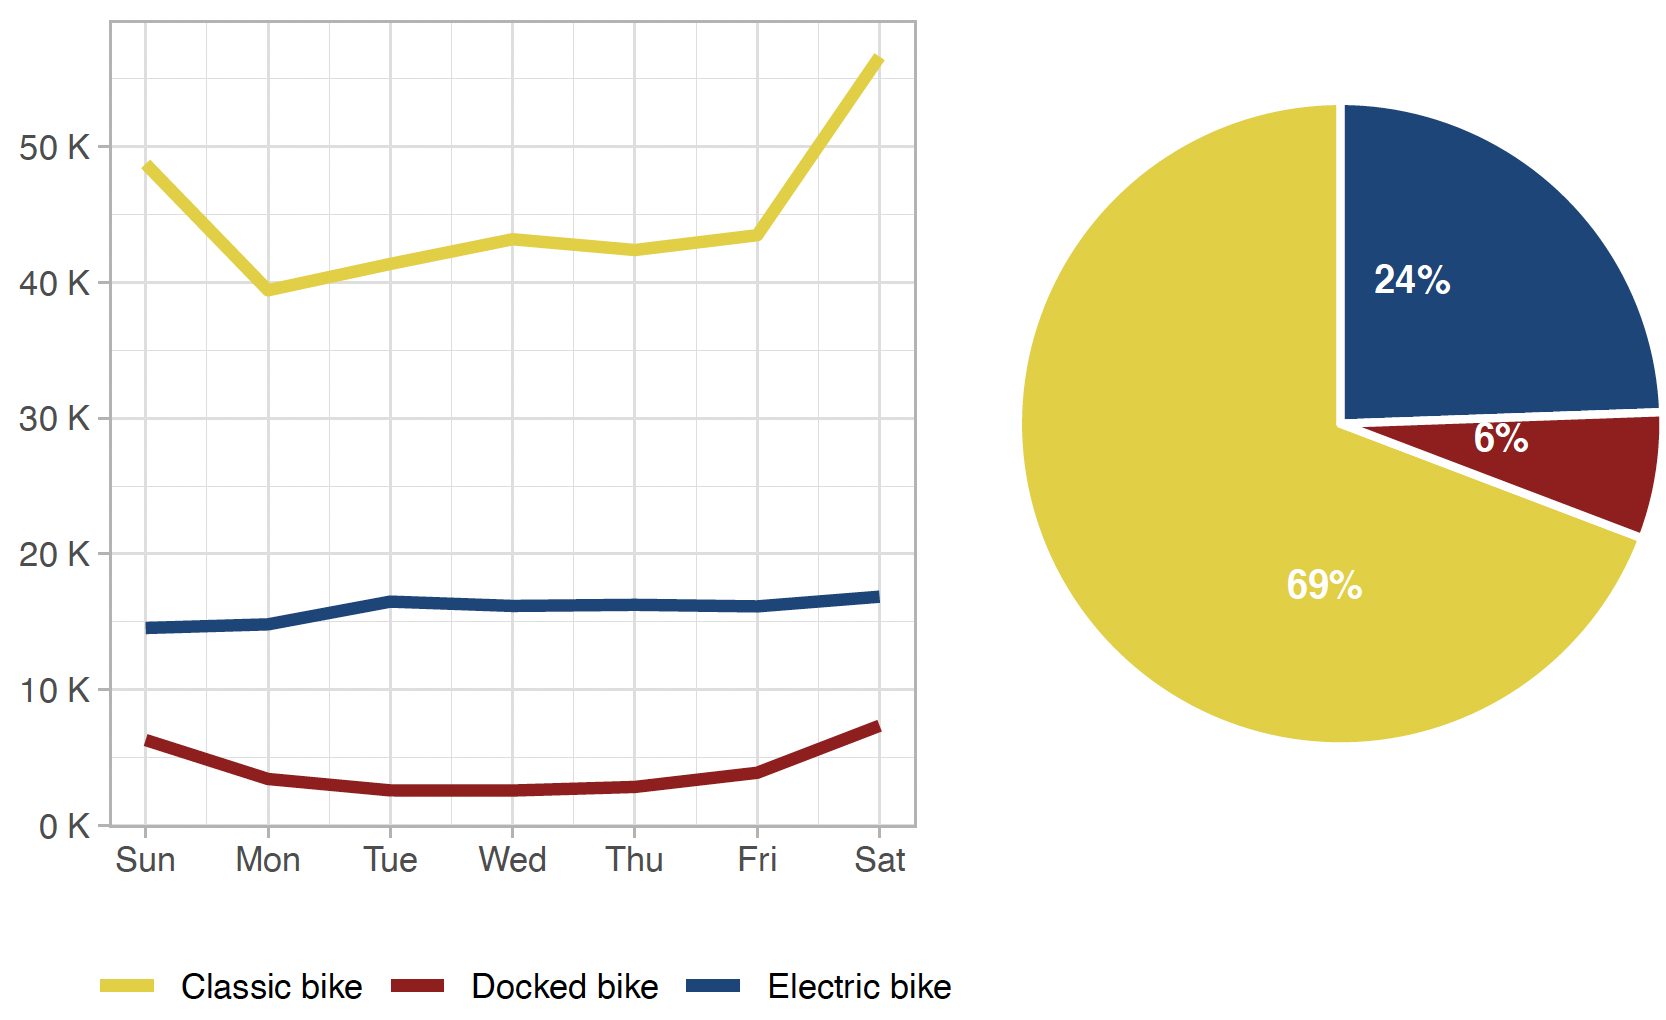
\includegraphics[width=11cm, height=7cm]{images/rideable-dayofweek}
	
\end{frame}
 	
   	\begin{frame}{Weekday versus Weekend Rides}
   	\centering
   	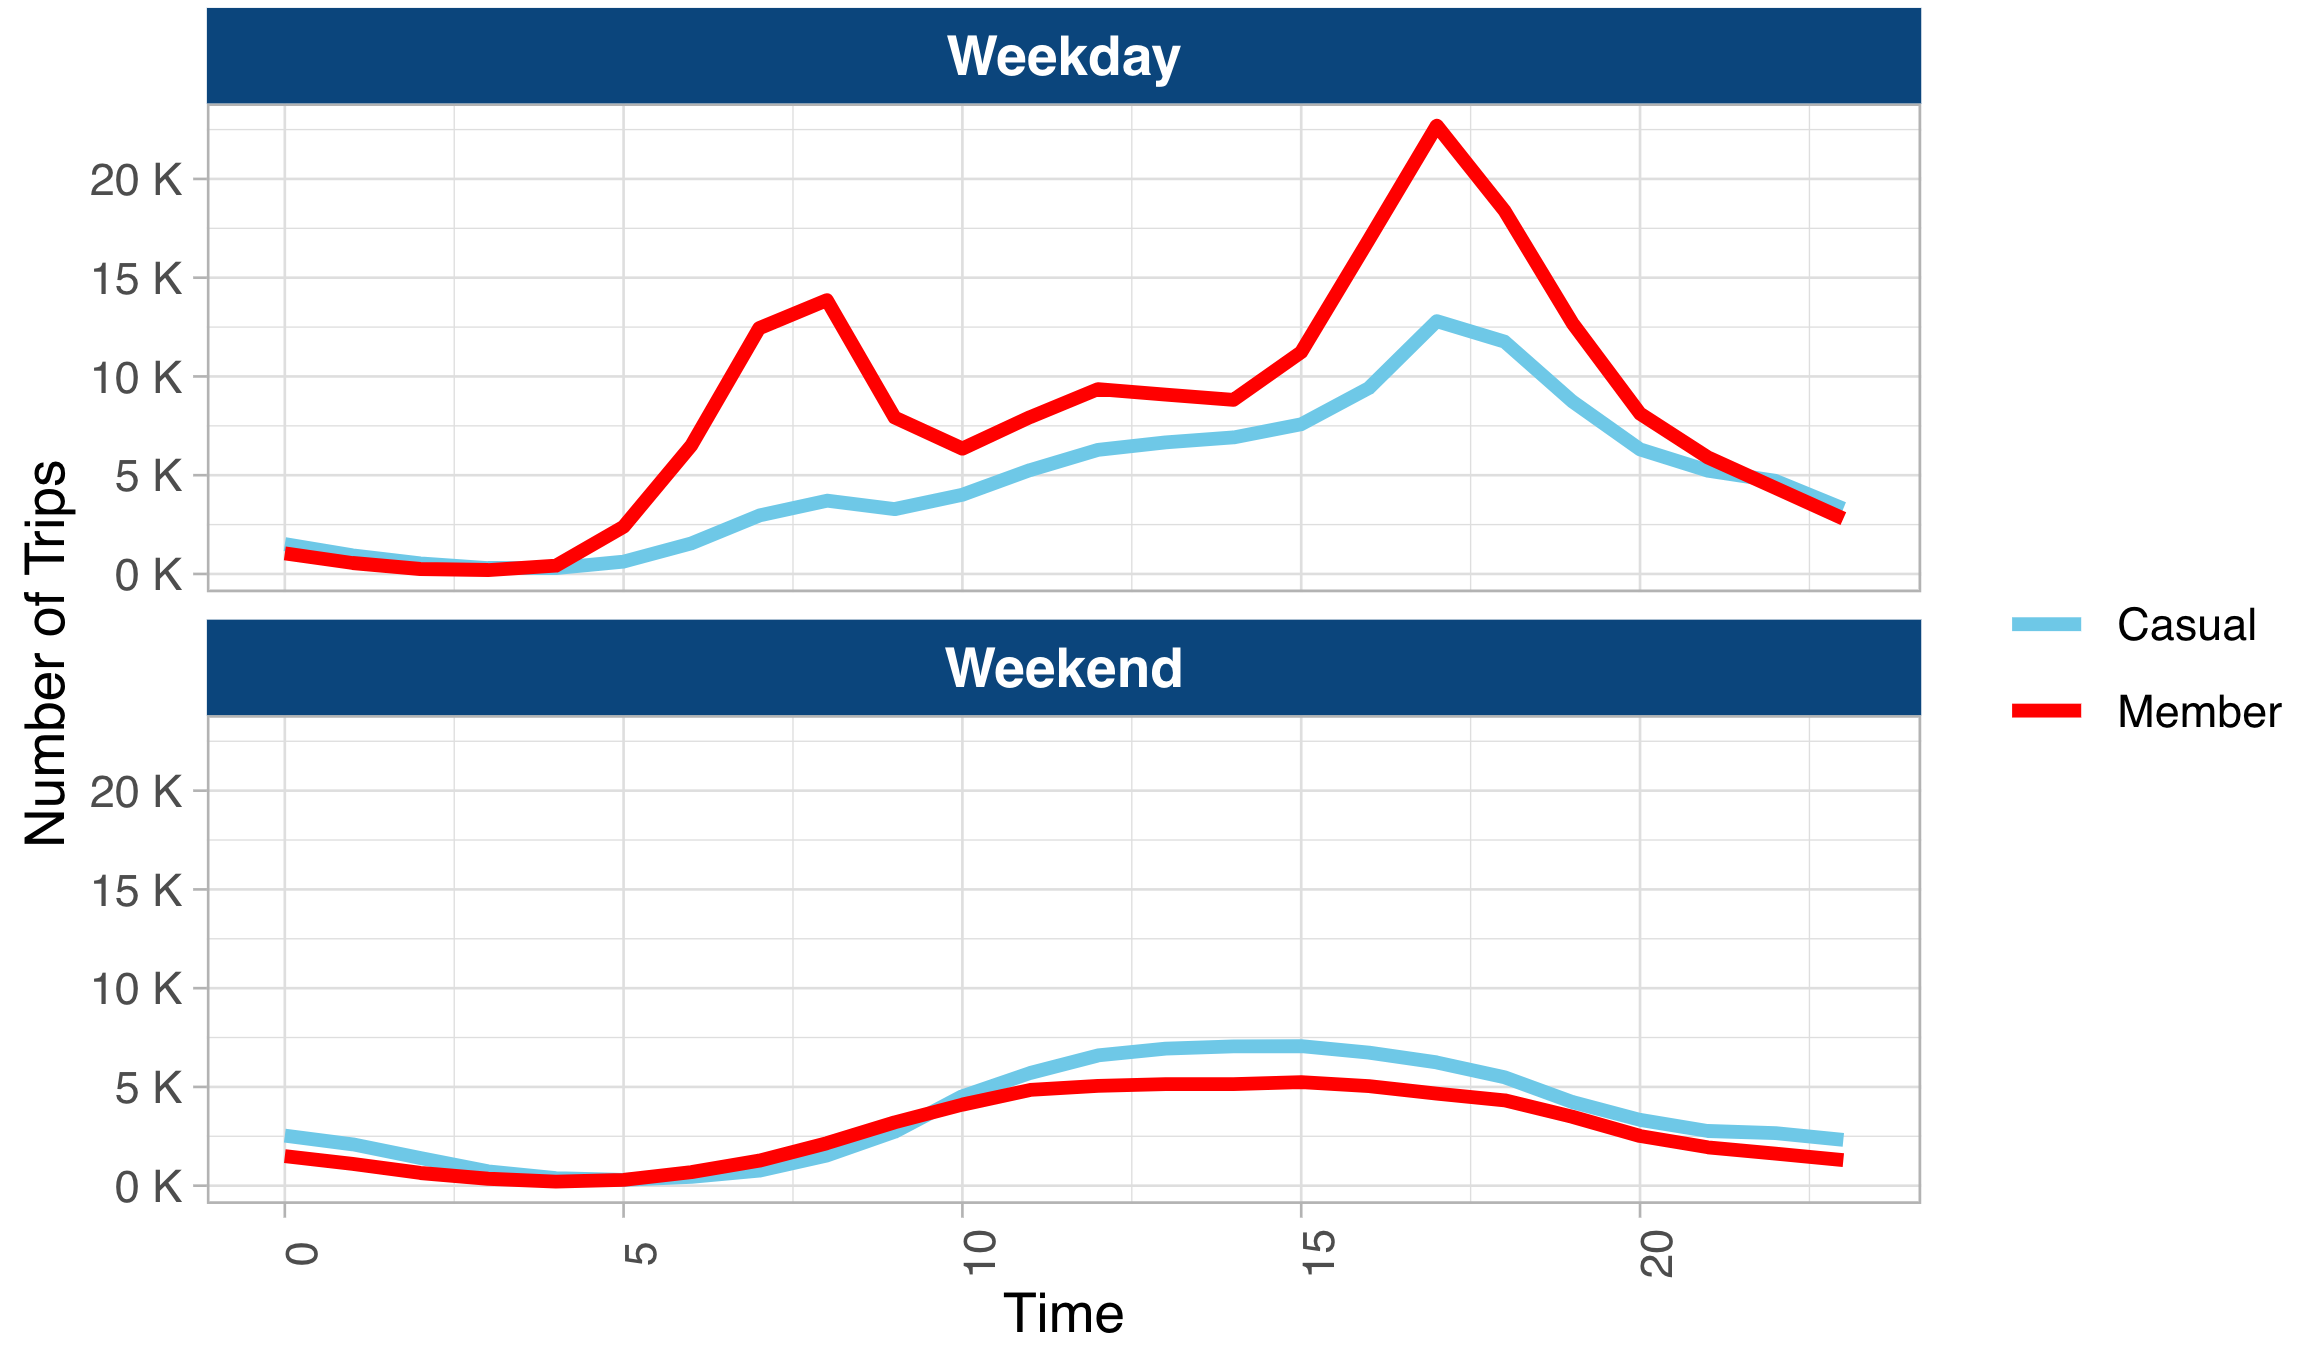
\includegraphics[width=11cm, height=7cm]{images/weekday-weekend}
   	
   \end{frame}

 	\begin{frame}{Weekday versus Weekend Rides}
	\centering
	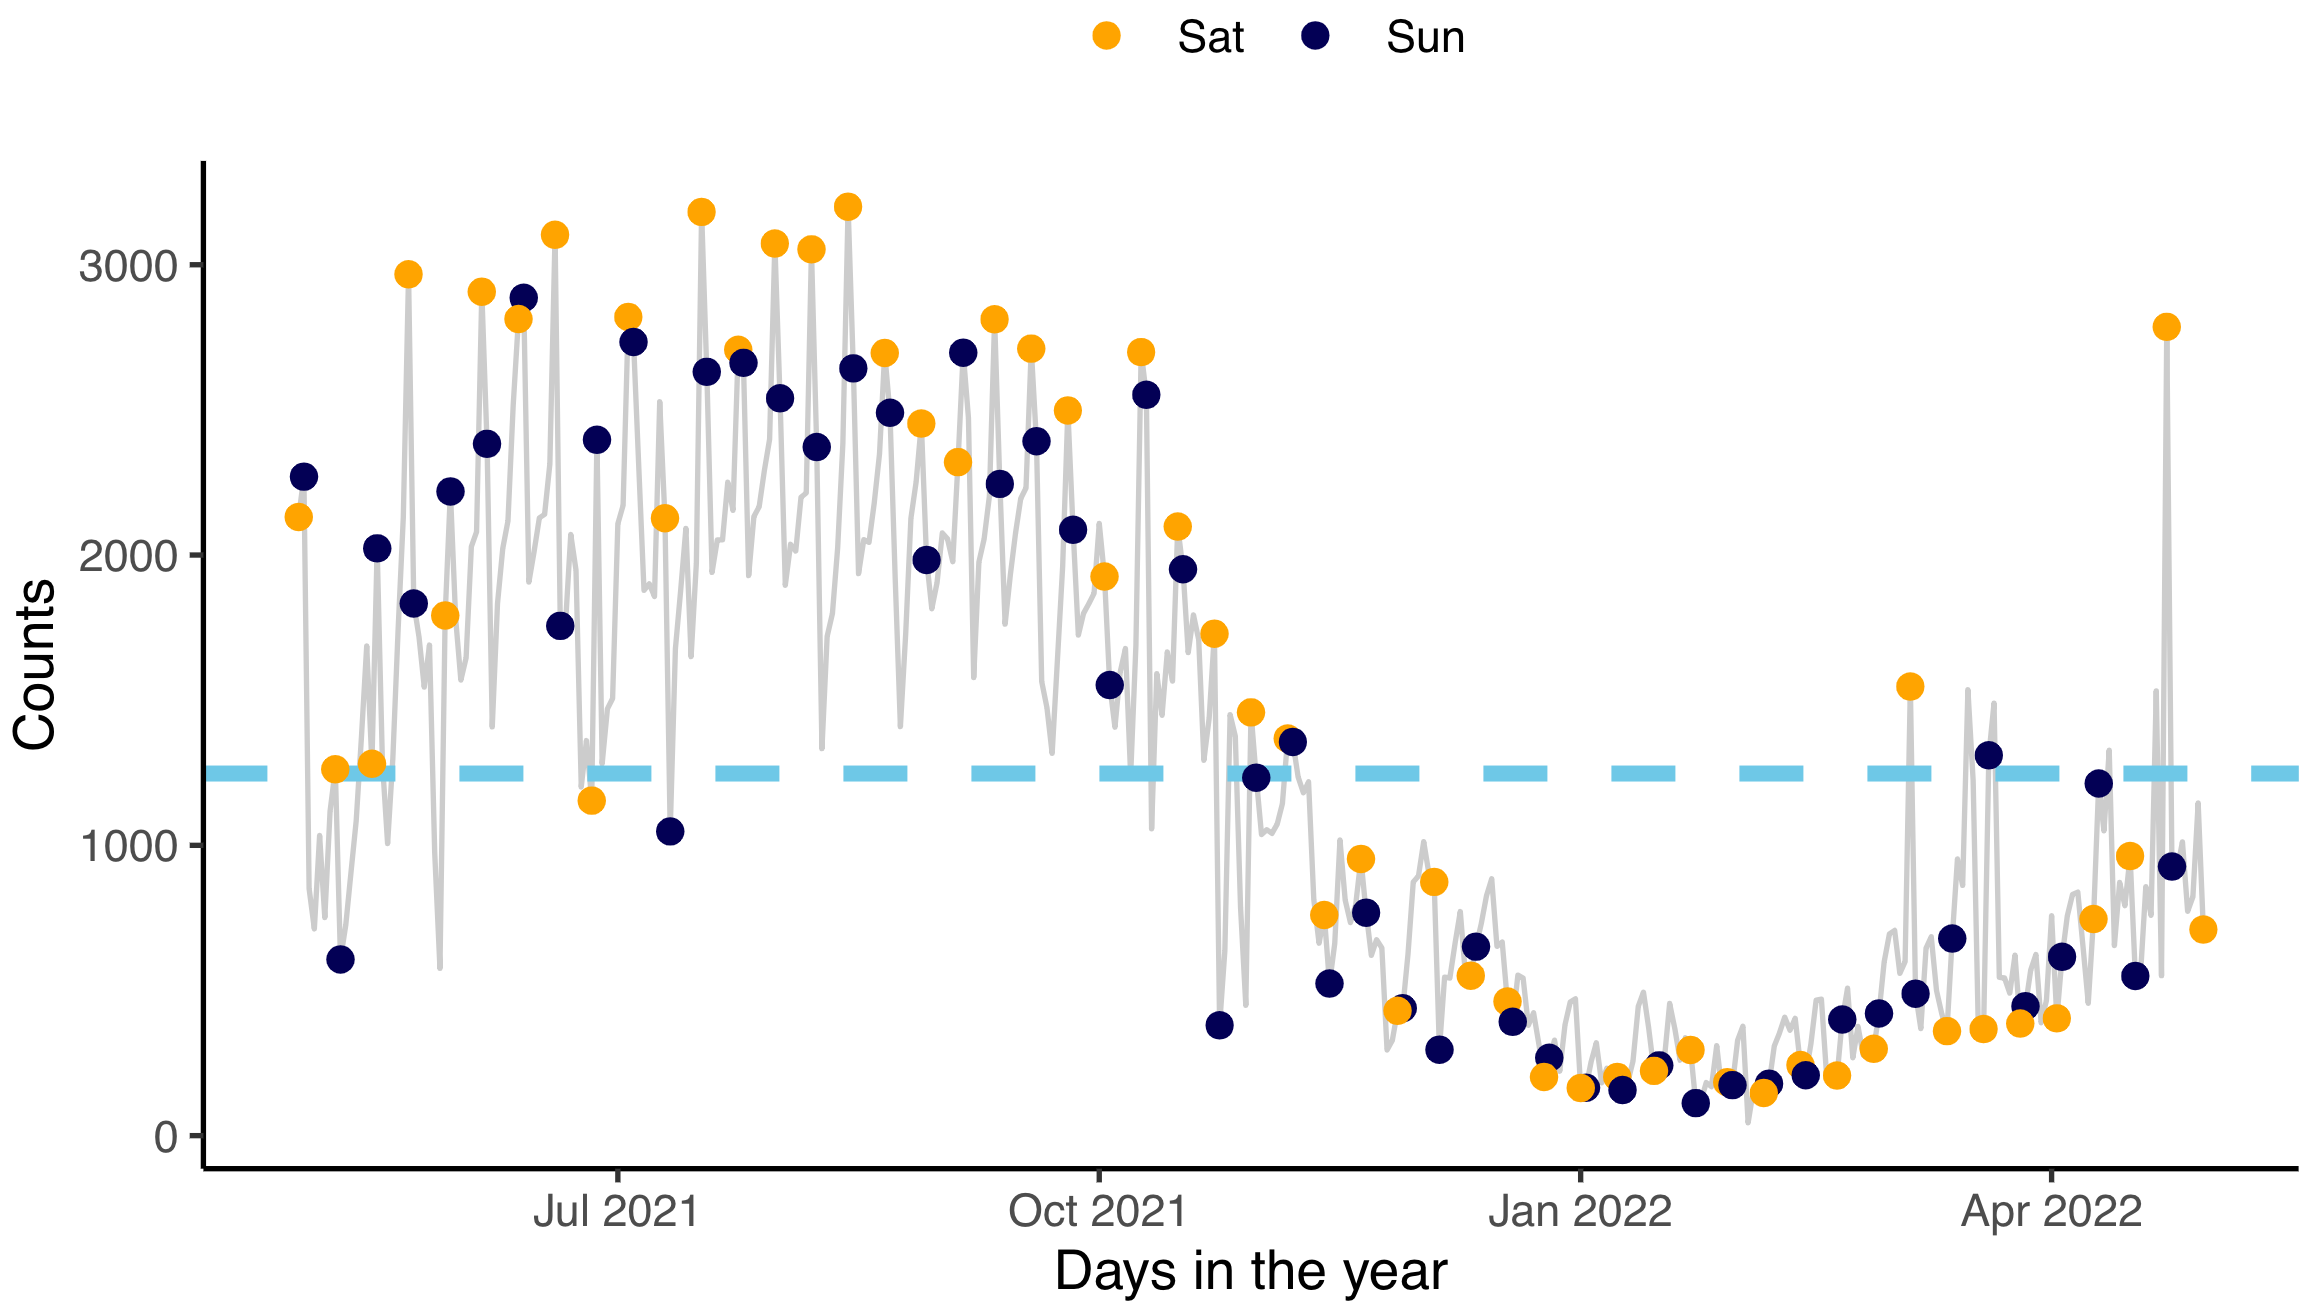
\includegraphics[width=11cm, height=7cm]{images/daily-year}
	
\end{frame}

\begin{frame}{Network Construction and Characteristics}
	
		\centering
	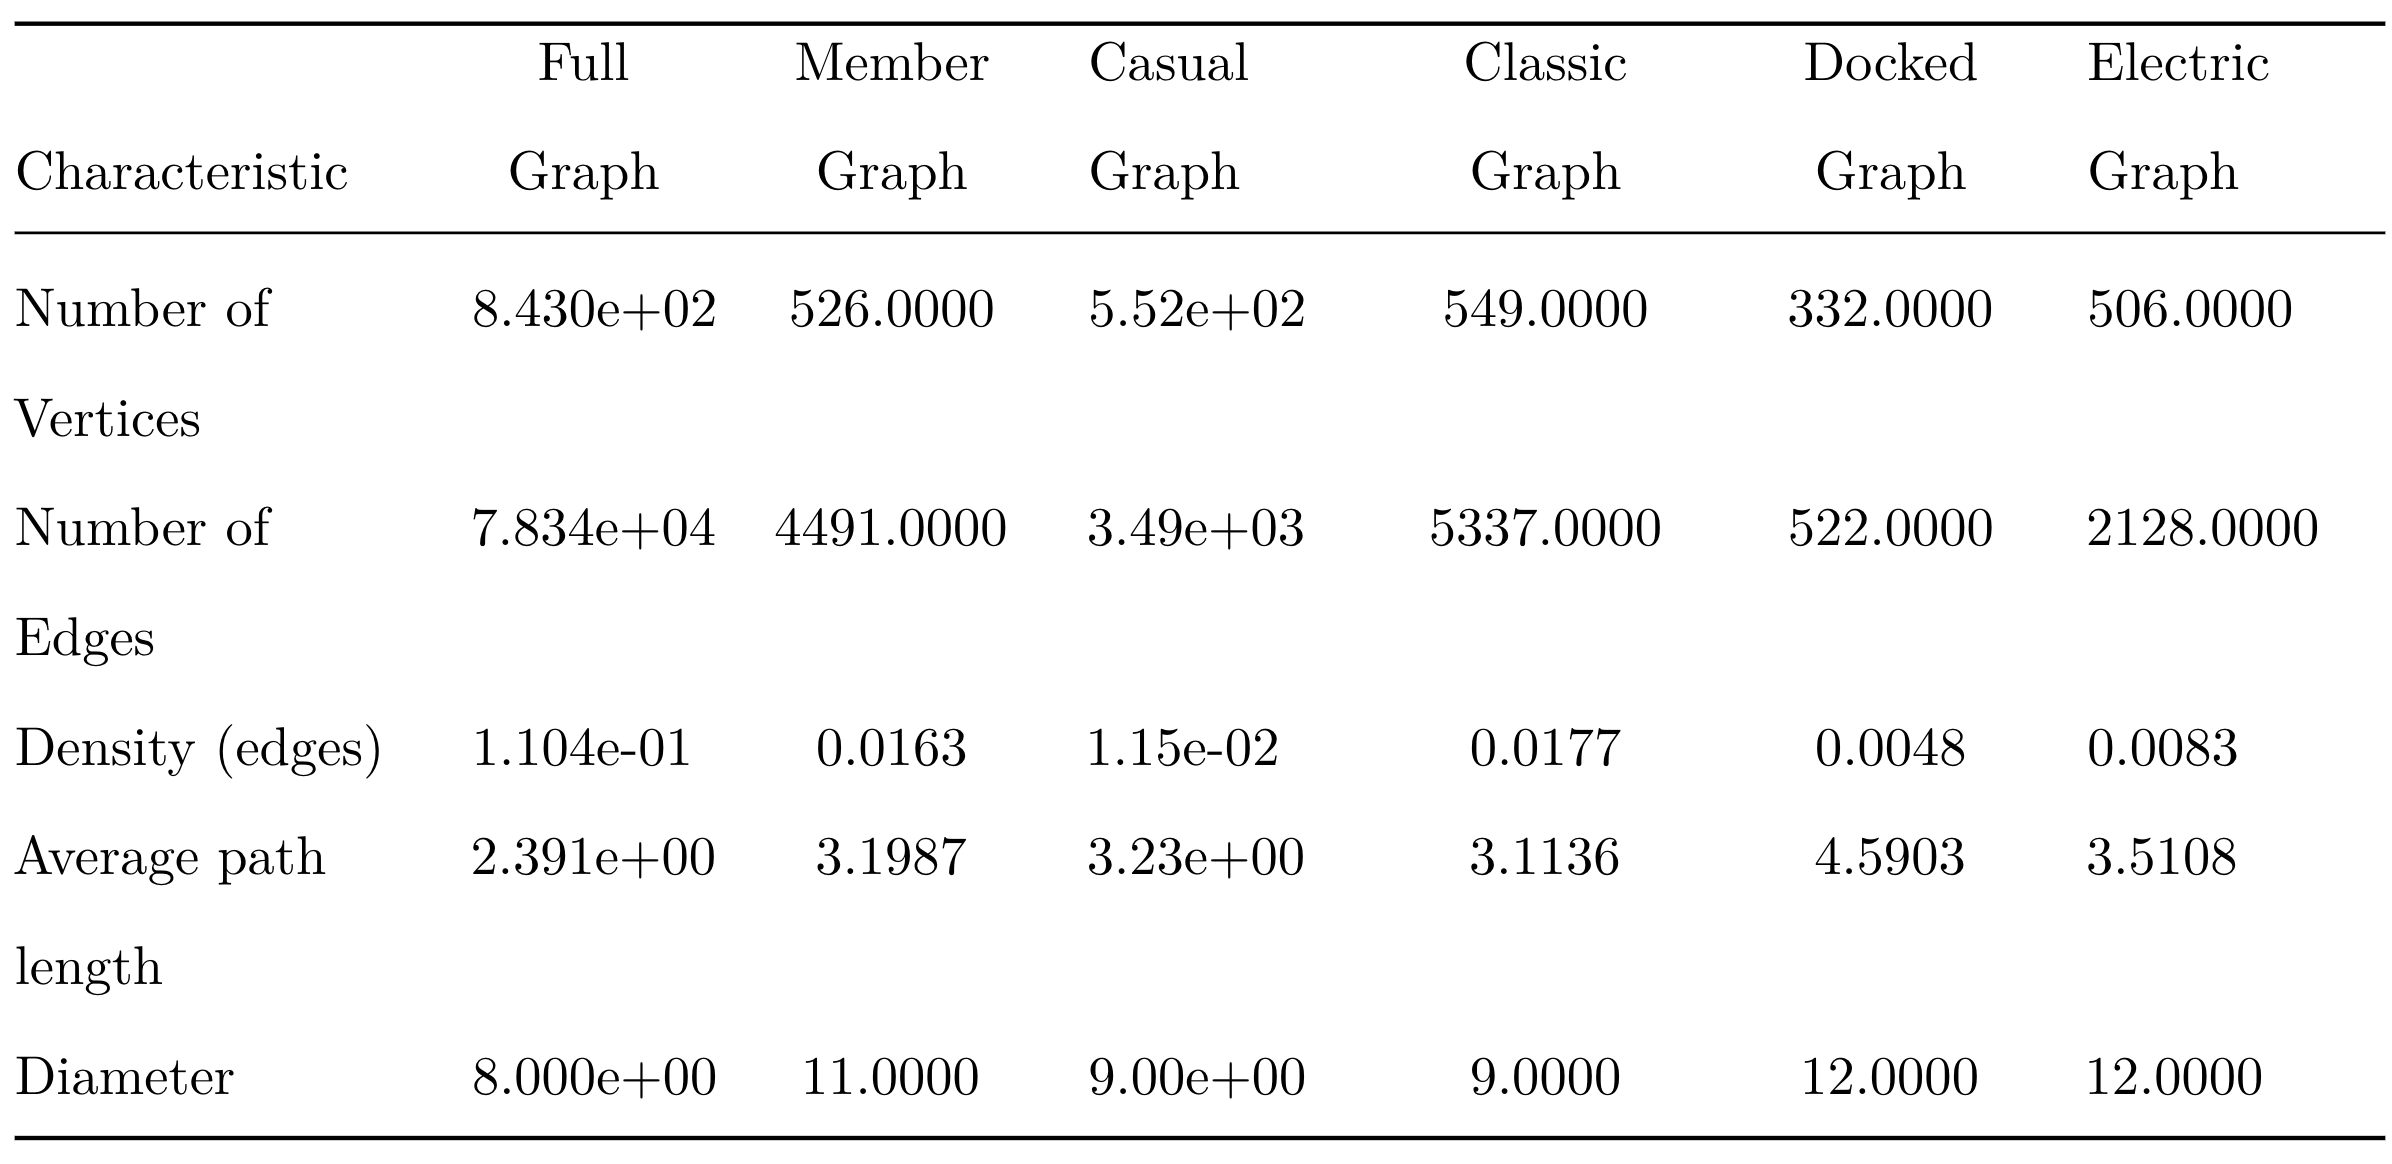
\includegraphics[width=10cm, height=7cm]{images/net-characteristics}
\end{frame}

\begin{frame}{User Type Graphs}
	
	\centering
	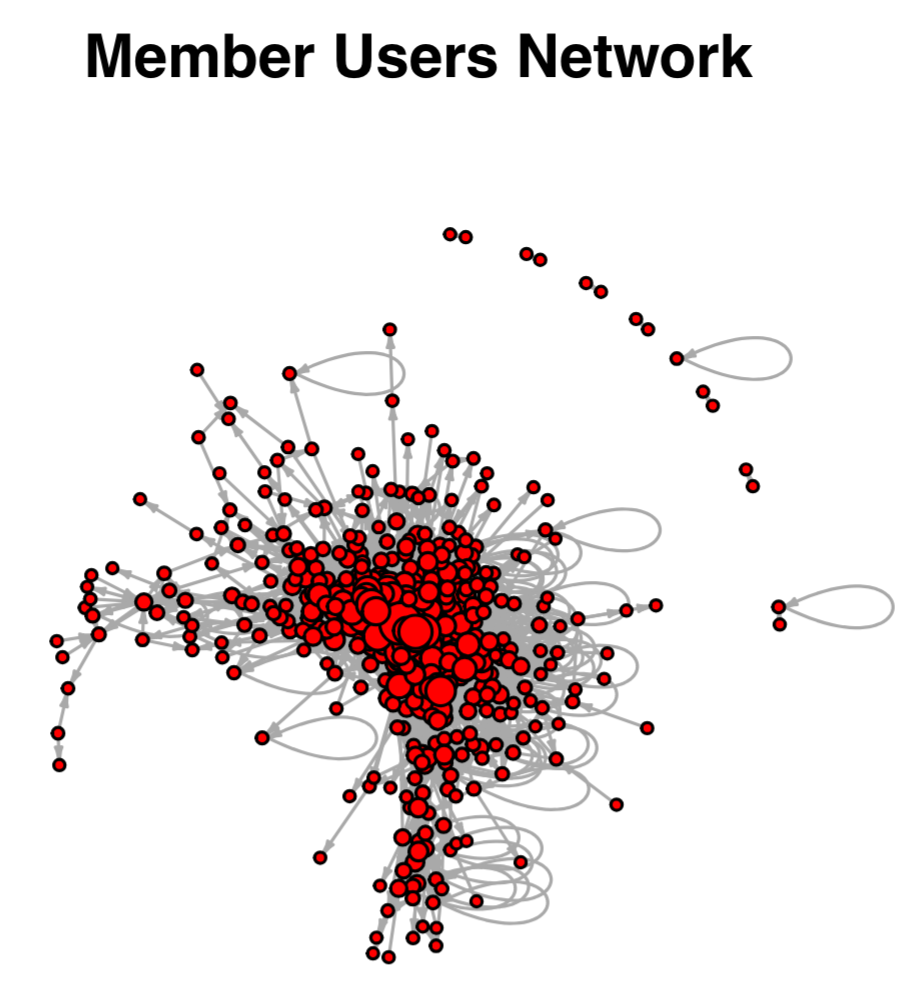
\includegraphics[width=10cm, height=7cm]{images/member-graph}
	
\end{frame}

\begin{frame}{User Type Graphs}
	
	\centering
	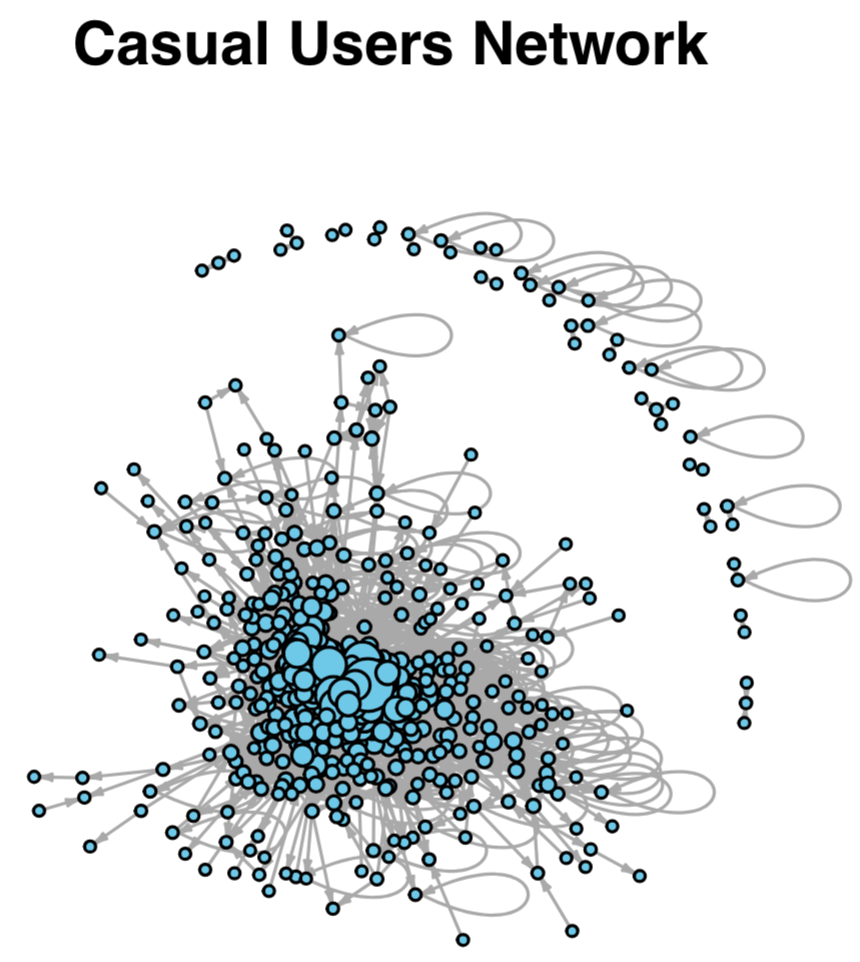
\includegraphics[width=10cm, height=7cm]{images/casual-graph}
	
\end{frame}

\begin{frame}{Ranking By Centrality Measures}
	
	\centering
	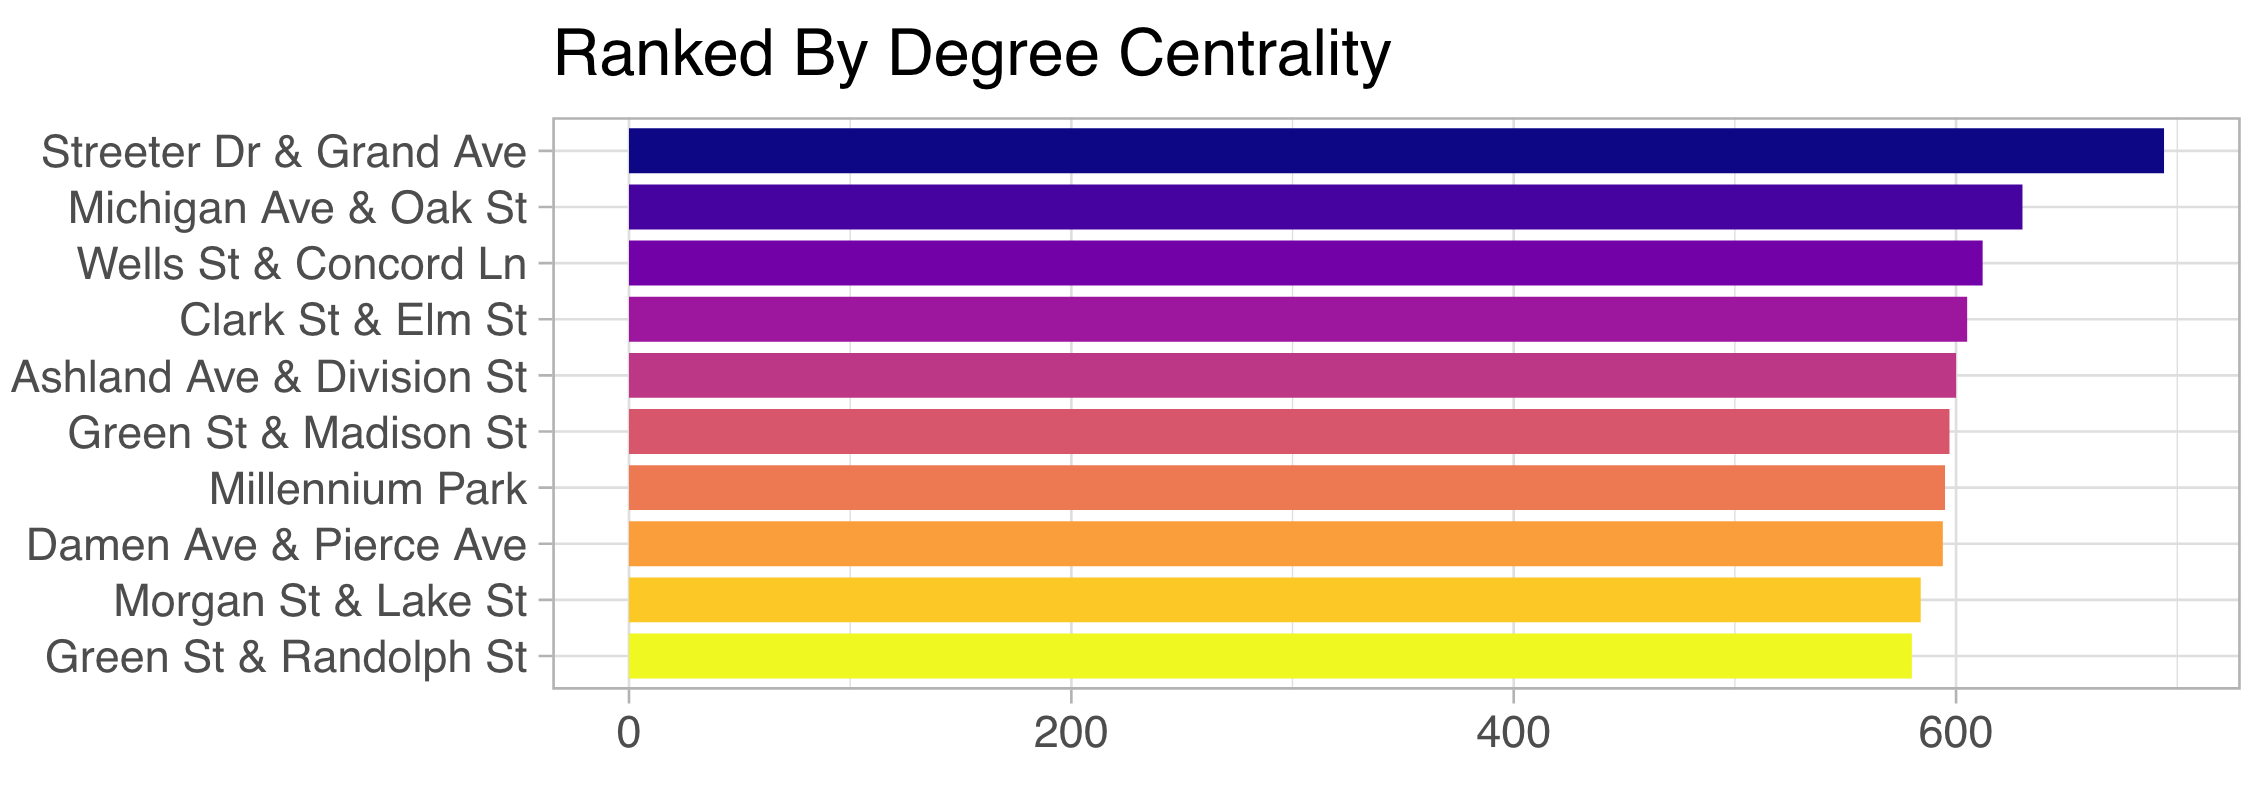
\includegraphics[width=10cm, height=7cm]{images/degree-ranking}
	
\end{frame}

\begin{frame}{Ranking By Centrality Measures}
	
	\centering
	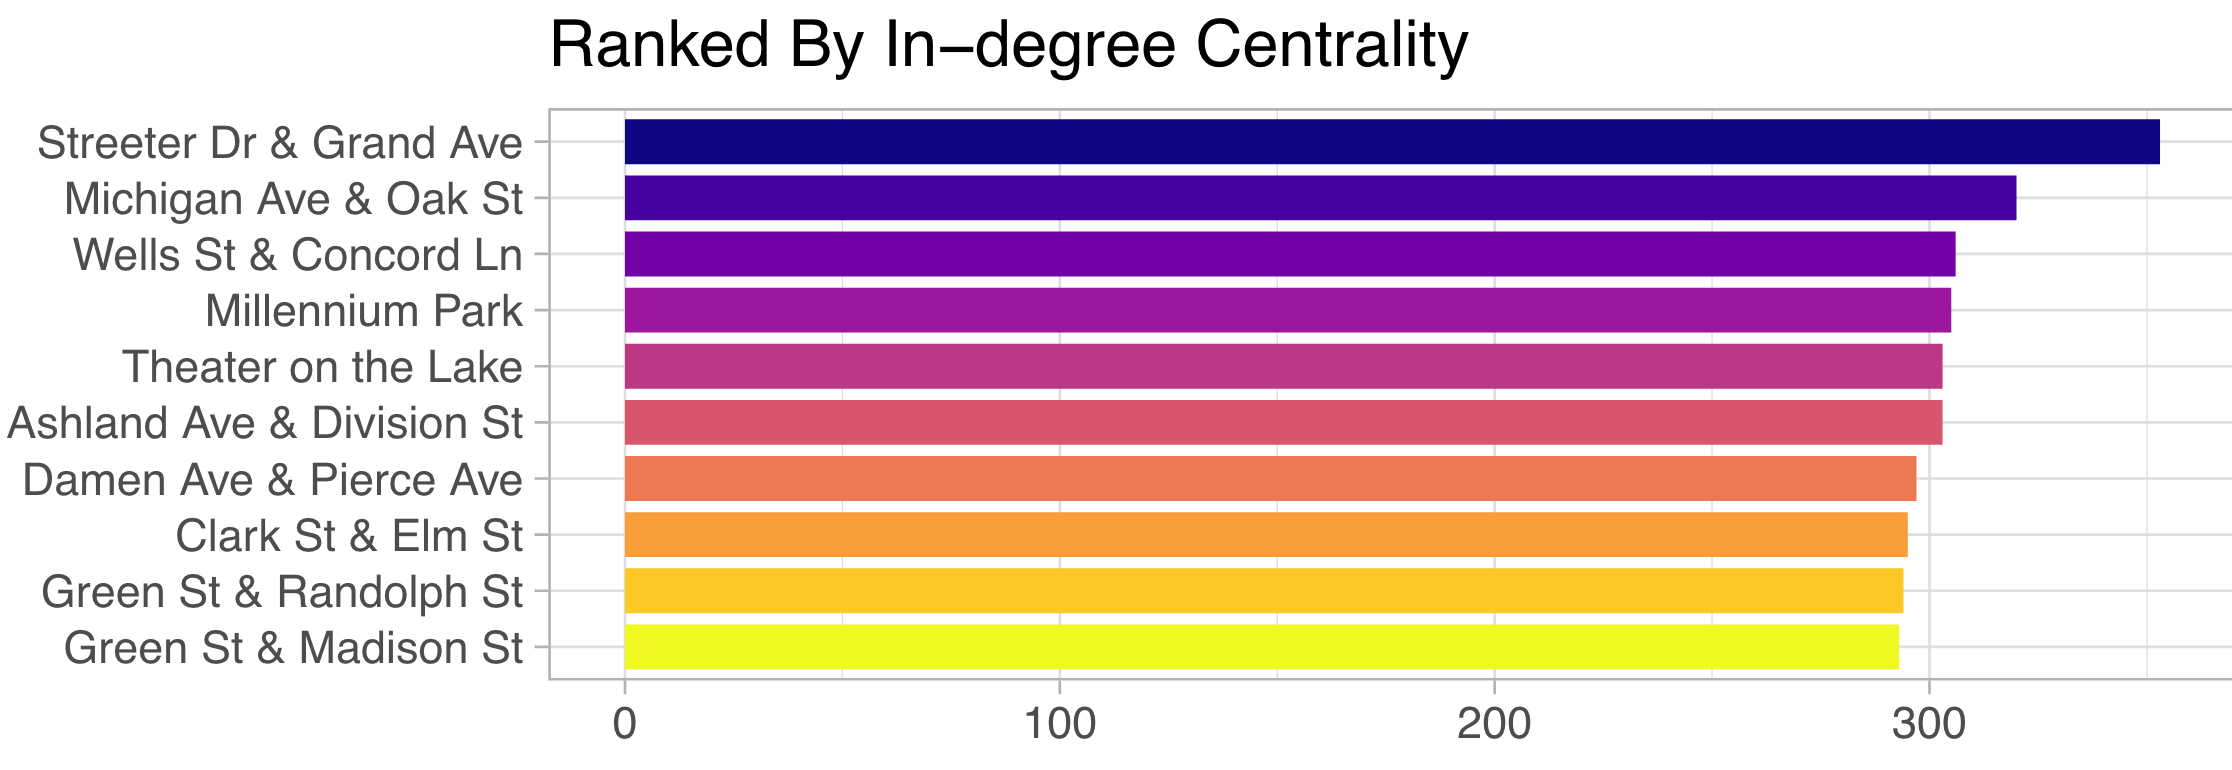
\includegraphics[width=10cm, height=7cm]{images/indegree-ranking}
	
\end{frame}

\begin{frame}{Ranking By Centrality Measures}
	
	\centering
	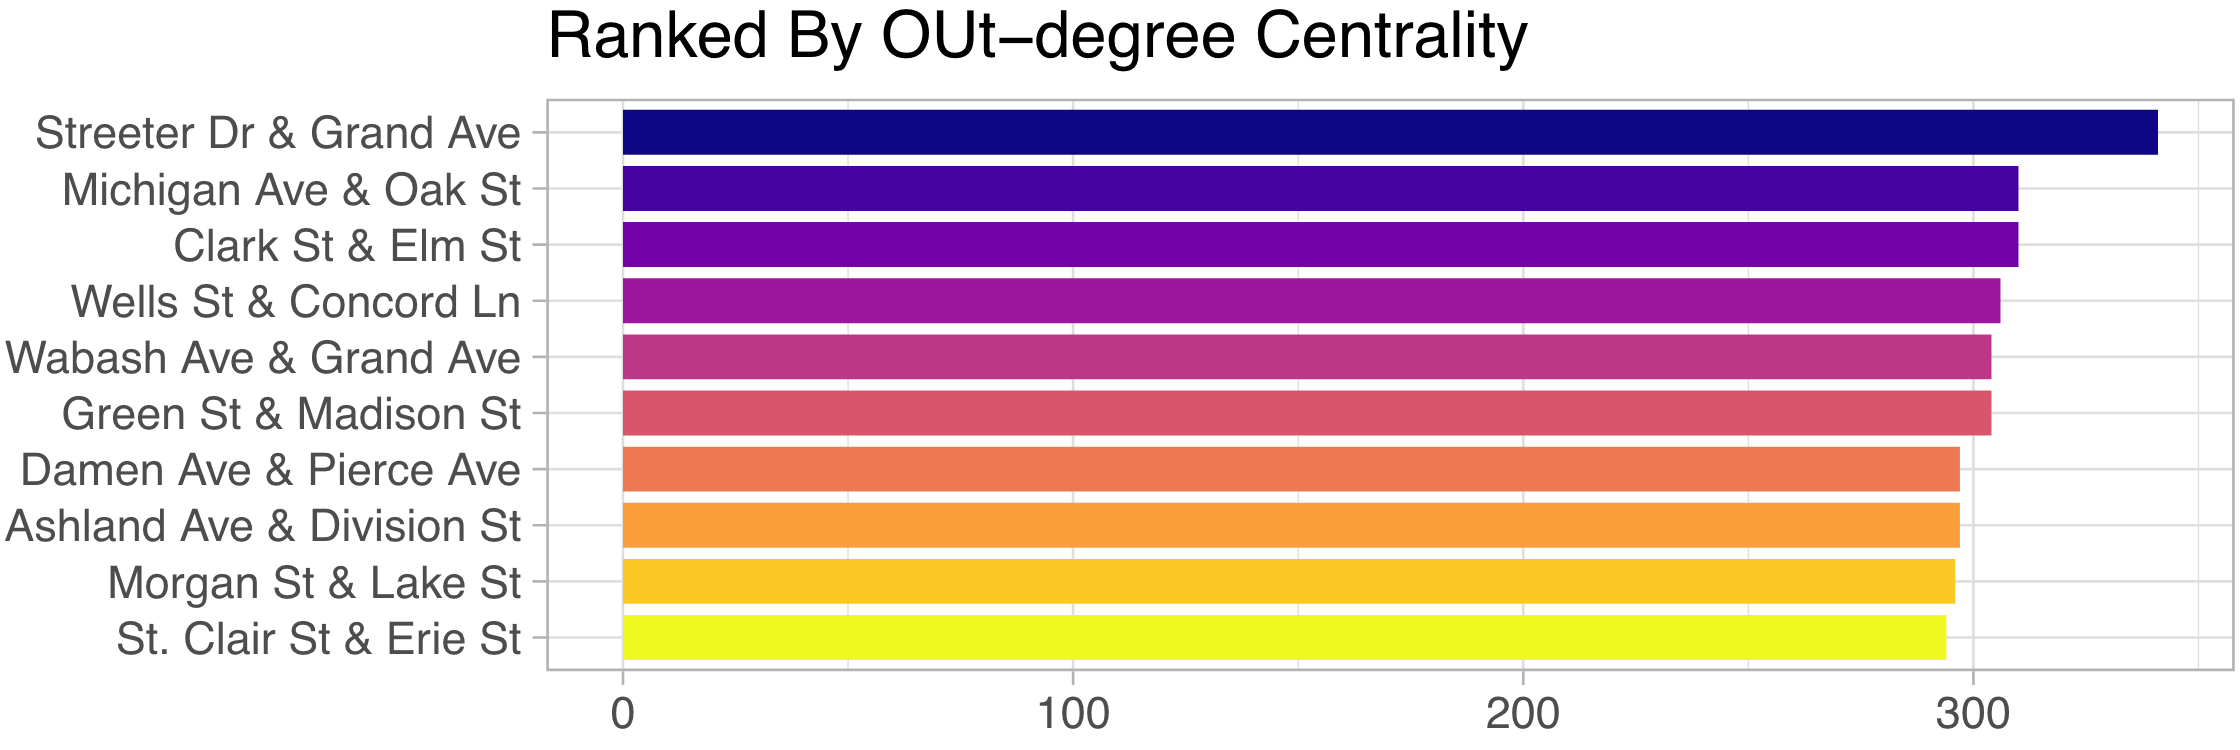
\includegraphics[width=10cm, height=7cm]{images/outdegree-ranking}
	
\end{frame}

\begin{frame}{Ranking By Centrality Measures}
	
	\centering
	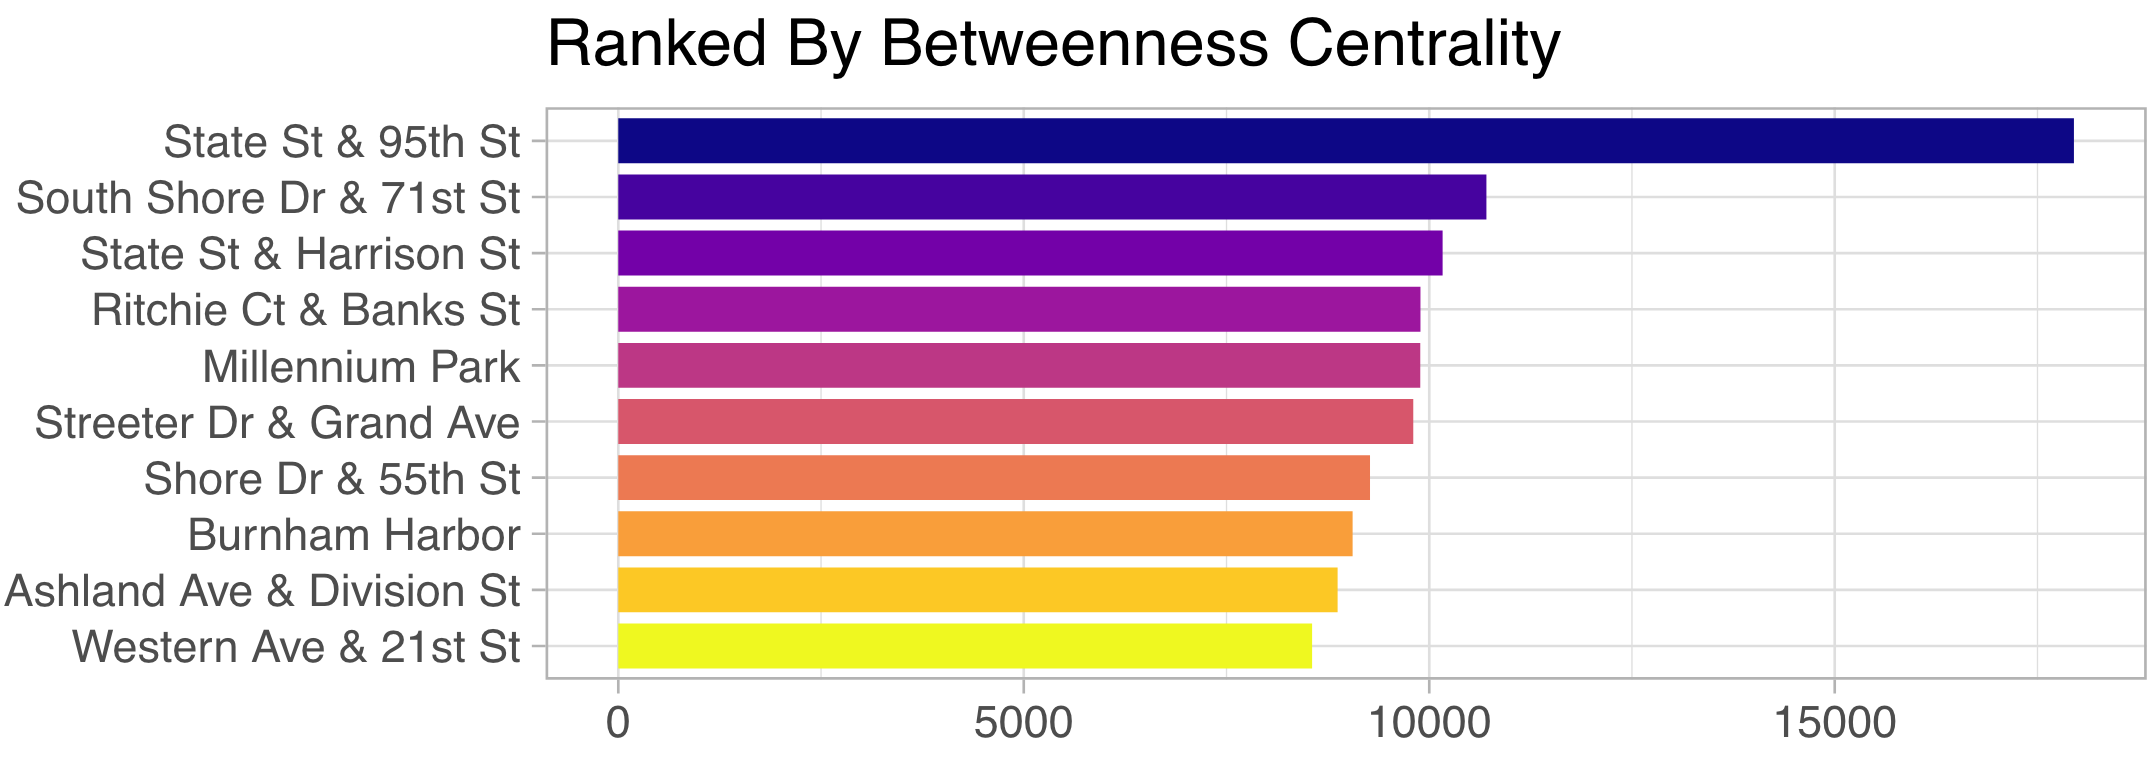
\includegraphics[width=10cm, height=7cm]{images/betweenness-ranking}
	
\end{frame}

\begin{frame}{Community Detection}
	
	\centering
	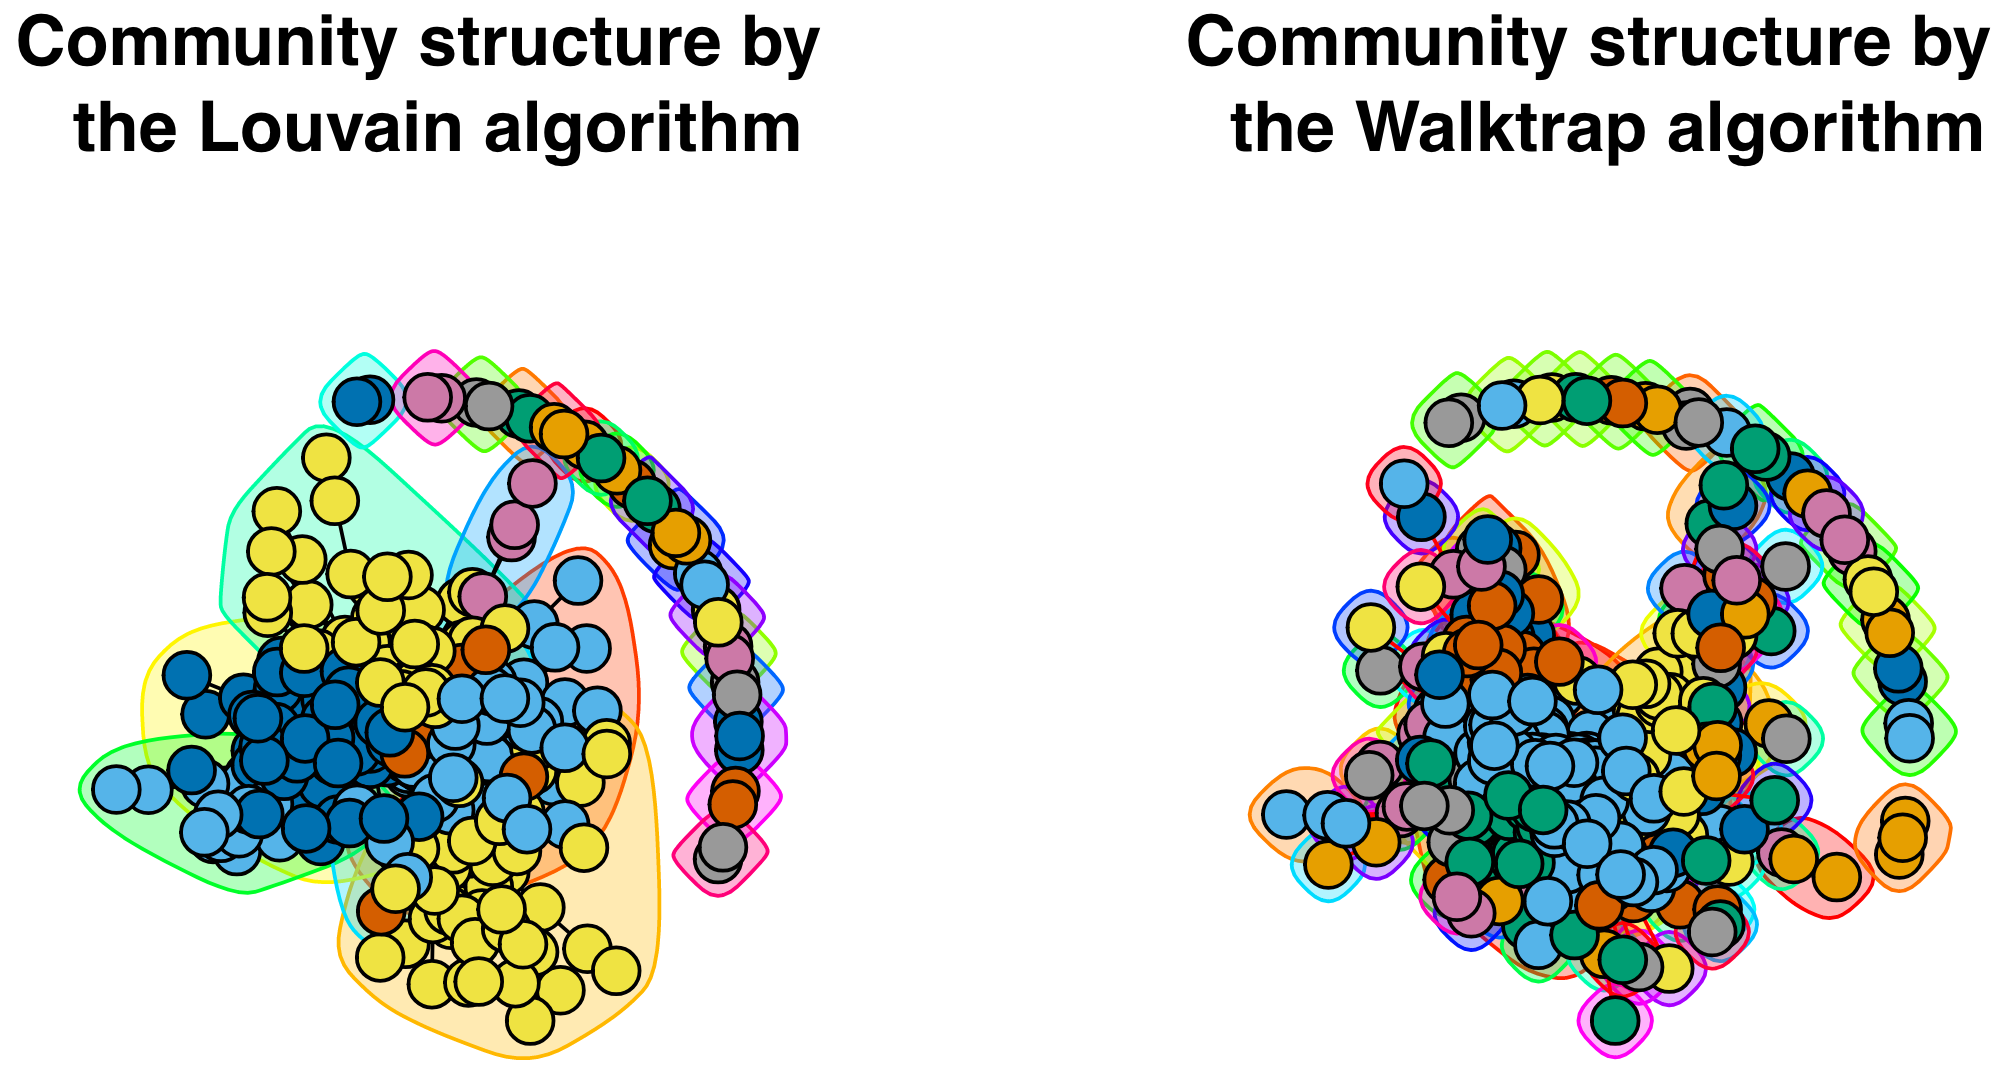
\includegraphics[width=10cm, height=7cm]{images/community-detection}
	
\end{frame}
\section{Discussion}

  \begin{frame}{Discussion}
  	\begin{itemize}
%  		\item Bike share users in Chicago use bike share for both one-way trips and round trips, but mostly one-way trips, and throughout the weekdays and on weekends
  		\item  Casual users make more rides on weekends than on weekdays and vice versa for members. 
%  		\item There were many Divvy bike-share stations with low usage of public bikes.
  		\item The analysis revealed that the \textbf{Streeter Dr \& Grand Avenue }bike station is the most central station
  		\item while the \textbf{State St \& 95th St }station appeared to be the most critical to information flow in the bike-share network.  
  		\item The bike-share network can be thought of as involving one big giant component 
  		
%  		which suggests that similar strategies can be adopted to bring improvement in ridership across all or most of the stations.
  		
%  		In this project I explored a 12-month sample of bike-share data from the Divvy bike-sharing system in Chicago and incorporated network analysis of the data to identify key stations and community structures. As a result of the large size of data obtained for just one year, a $10\%$ stratified random sample was drawn to ease computational burden without compromising the representativeness of the data population. 
  	\end{itemize}
  \end{frame}

\section{Limitations}
\begin{frame}
	\begin{itemize}
		\item The study was largely plagued by limited time constraint
		\item Failure to explore spatial trends
		\item Lack of demographic and weather information
	\end{itemize}
\end{frame}
 \begin{frame}{Reference}
 	\begin{itemize}
 	 \item Rixey, R. A. (2013). Station-level forecasting of bikesharing ridership: Station network effects in three US systems. Transportation research record, 2387(1), 46-55.
 	
 	\item Yao, Y., Zhang, Y., Tian, L., Zhou, N., Li, Z., \& Wang, M. (2019). Analysis of network structure of urban bike-sharing system: A case study based on real-time data of a public bicycle system. Sustainability, 11(19), 5425.tical model to analyze COVID-19 spread in the USA." Journal of Applied Statistics (2021): 1-20.
 	\end{itemize}
 \end{frame}

%	\section{Conclusion}
	
	\section*{Reference}
\end{document}